\documentclass[a4paper,12pt]{article} % добавить leqno в [] для нумерации слева
\usepackage[a4paper,top=1.3cm,bottom=2cm,left=1.5cm,right=1.5cm,marginparwidth=0.75cm]{geometry}
%%% Работа с русским языком
\usepackage{cmap}					% поиск в PDF
\usepackage{mathtext} 				% русские буквы в фомулах
\usepackage[T2A]{fontenc}			% кодировка
\usepackage[utf8]{inputenc}			% кодировка исходного текста
\usepackage[english,russian]{babel}	% локализация и переносы

\usepackage{graphicx}

\usepackage{wrapfig}
\usepackage{tabularx}

\usepackage{hyperref}
\usepackage[rgb]{xcolor}
\hypersetup{
colorlinks=true,urlcolor=blue
}
\usepackage{multirow}
\usepackage{hhline}


%%% Дополнительная работа с математикой
\usepackage{amsmath,amsfonts,amssymb,amsthm,mathtools} % AMS
\usepackage{icomma} % "Умная" запятая: $0,2$ --- число, $0, 2$ --- перечисление

%% Номера формул
\mathtoolsset{showonlyrefs=true} % Показывать номера только у тех формул, на которые есть \eqref{} в тексте.

%% Шрифты
\usepackage{euscript}	 % Шрифт Евклид
\usepackage{mathrsfs} % Красивый матшрифт

%% Свои команды
\DeclareMathOperator{\sgn}{\mathop{sgn}}

%% Перенос знаков в формулах (по Львовскому)
\newcommand*{\hm}[1]{#1\nobreak\discretionary{}
{\hbox{$\mathsurround=0pt #1$}}{}}

\begin{document}
	
	\begin{titlepage}
	\begin{center}
		{\large МОСКОВСКИЙ ФИЗИКО-ТЕХНИЧЕСКИЙ ИНСТИТУТ (НАЦИОНАЛЬНЫЙ ИССЛЕДОВАТЕЛЬСКИЙ УНИВЕРСИТЕТ)}
	\end{center}
	\begin{center}
		{\large Физтех-школа электроники, фотоники и молекулярной физики}
	\end{center}
	
	
	\vspace{4.5cm}
	{\huge
		\begin{center}
			{Лабораторная работа 4.2.1}\\
			Кольца Ньютона
		\end{center}
	}
	\vspace{2cm}
	\begin{flushright}
		{\LARGE Салтыкова Дарья \\
			\vspace{0.5cm}
			Б04-105}
	\end{flushright}
	\vspace{8cm}
	\begin{center}
		Долгопрудный 2023
	\end{center}
\end{titlepage}

\section{Введение}

\noindent \textbf{Цель работы:} познакомиться с явлением интерференции в тонких плёнках (полосы равной толщины) на примере колец Ньютона и с методикой интерференционных измерений кривизны стеклянной поверхности.
	 

\medskip
	
\noindent \textbf{В работе используются:} измерительный микроскоп с опак-иллюминатором, плоско-выпуклая линза; пластинка из чёрного стекла, ртутная лампа типа ДРШ, щель, линзы, призма прямого зрения, объектная шкала.
	

\section{Теоретические сведения}

		\begin{figure}[h!]
 	\centering 	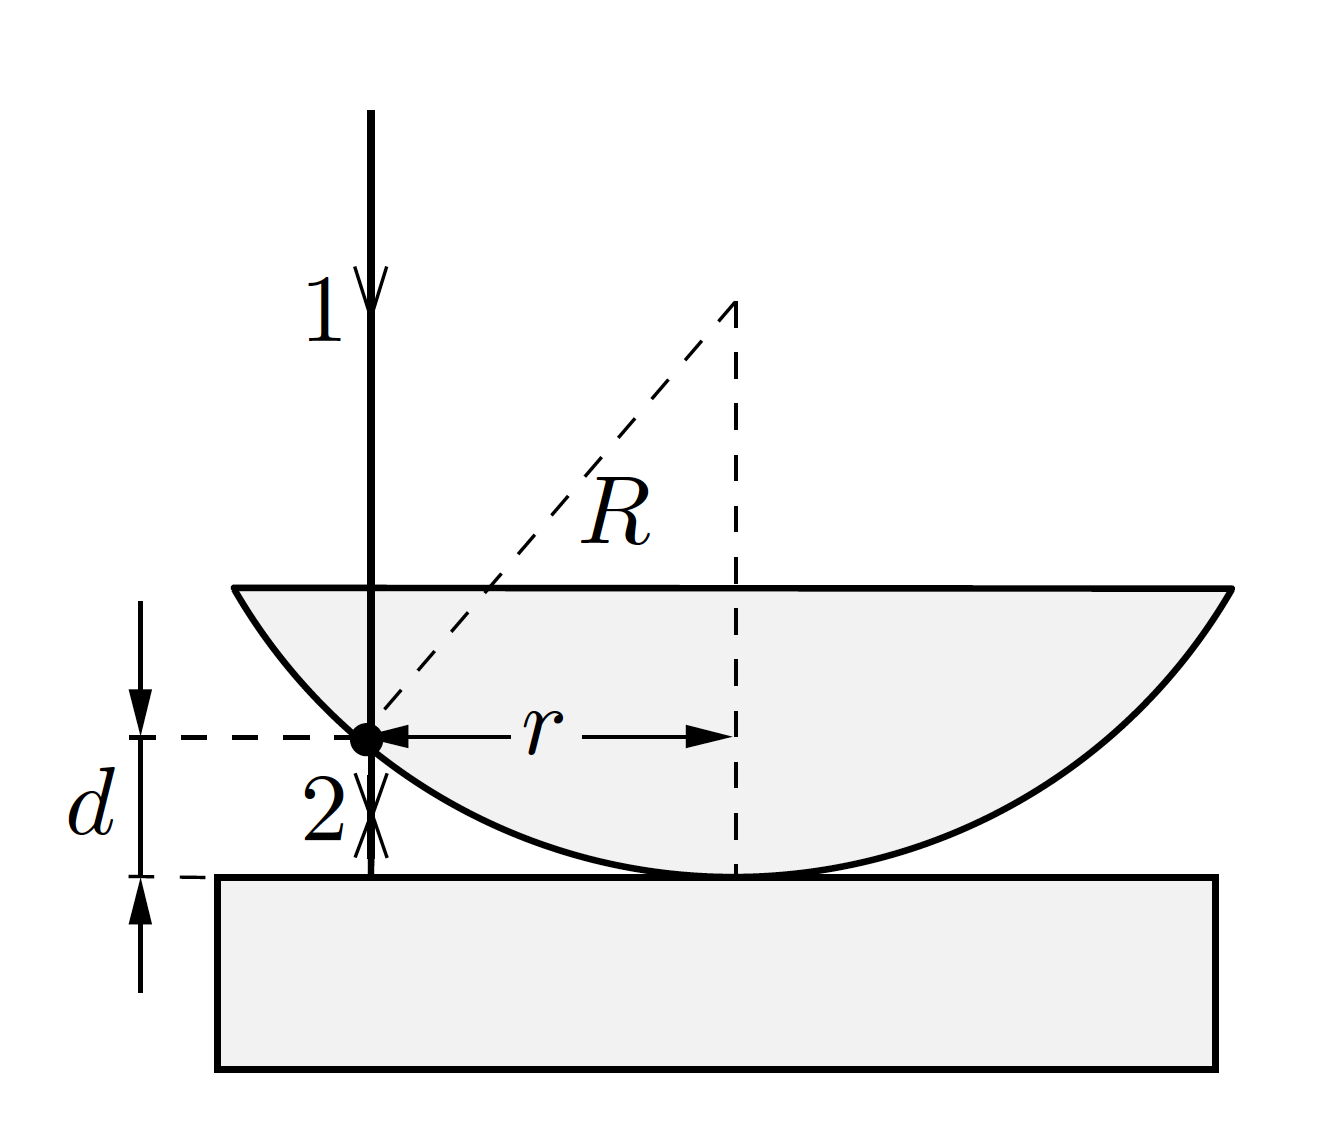
\includegraphics[width=0.4\linewidth]{ring.png}
 \end{figure}



\noindent Этот классический опыт используется для определения радиуса кривизны сферических поверхностей линз. В этом опыте наблюдается интерференция волн, отражённых от границ тонкой воздушной прослойки, образованной сферической поверхностью линзы и плоской стеклянной пластиной. При нормальном падении света интерференционные полосы локализованы на сферической поверхности и являются полосами равной толщины.

\medskip
	
\noindent Геометрическая разность хода между интерферирующими лучами равна удвоенной толщине воздушного зазора $ 2d $ в данном месте. Для точки на сферической поверхности, находящейся на расстоянии $ r $ от оси системы, имеем $ r^2 = R^2 - (R - d)^2 = 2Rd - d^2 $, где $ R $ --- радиус кривизны сферической поверхности.

\medskip
	
\noindent При $ R \gg d $ получим$  d = r^2/2R $. С учётом изменения фазы на $ \pi $ при отражении волны от оптически более плотной среды (на границе воздух-стекло) получим оптическую разность хода интерферирующих лучей:
	
	\begin{equation}\label{r_m}
	\Delta = \dfrac{\lambda}{2} + 2d = \dfrac{r^2}{2R} + \dfrac{\lambda}{2}
	\end{equation}
	
\noindent Из условия интерференционного минимума $ \Delta = \dfrac{(2m +1)\lambda}{2}, \; m =0, 1, 2.. $ получим радиусы темных колец $ r_m $, а из аналогичного условия максимума $ \Delta = m \lambda $ радиусы светлых $ r_m' $ :
	
	\begin{equation}\label{r_m'}
	r_m = \sqrt{m \lambda R}, \qquad 	r_m' = \sqrt{\dfrac{(2m-1)m \lambda R}{2}}
	\end{equation}
	
	\section{Экспериментальная установка}

\noindent Схема экспериментальной установки приведена на рисунке. Опыт выполняется с помощью измерительного микроскопа.
На столик микроскопа помещается держатель с полированной пластинкой из
чёрного стекла. На пластинке лежит исследуемая линза.

	\begin{wrapfigure}{r}{0.5\linewidth} 
	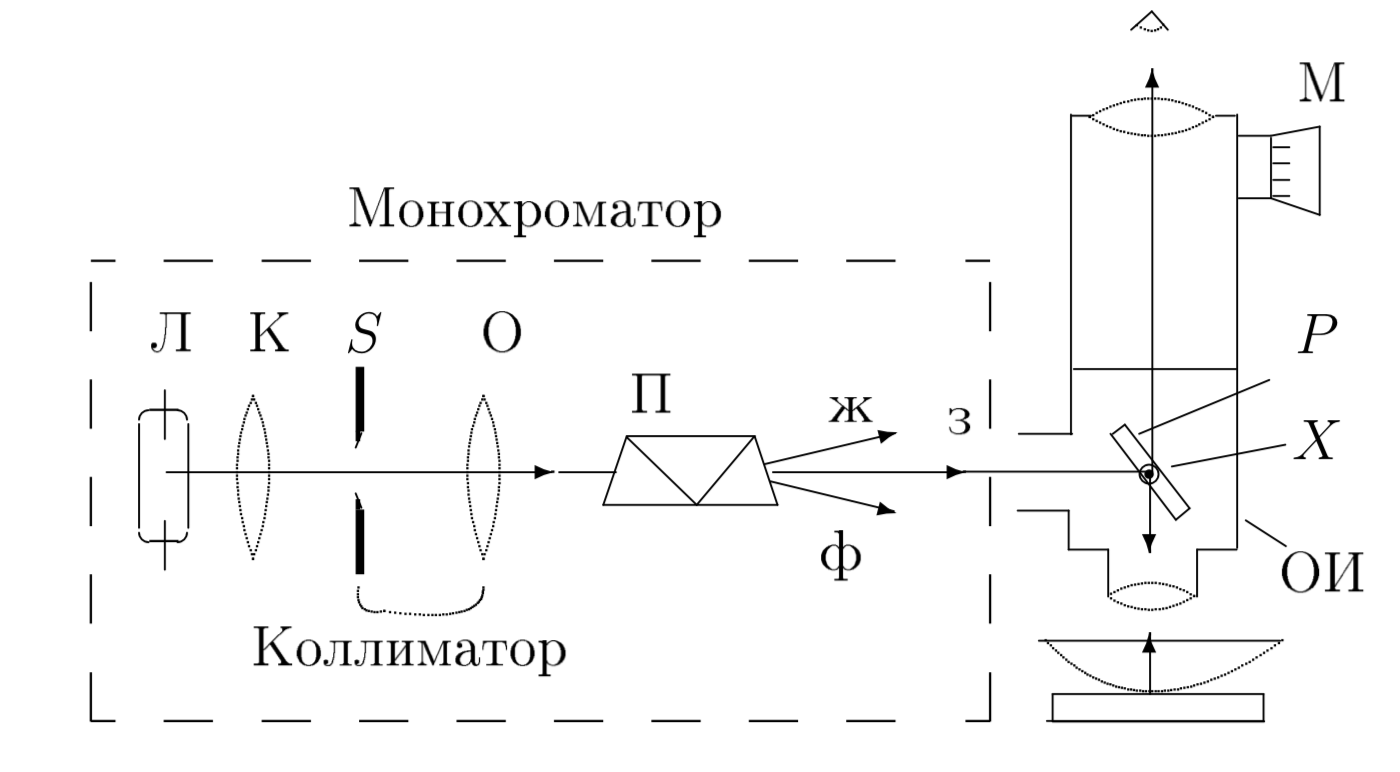
\includegraphics[width=\linewidth]{lab}
	\caption{Экспериментальная установка}
	\label{lab}
\end{wrapfigure}

\medskip

\noindent Источником света служит ртутная лампа, находящаяся в защитном кожухе. Для получения монохроматического света применяется призменный монохроматор, состоящий из конденсора $ К $, коллиматора (щель $ S $ и объектив $ О $) и призмы прямого зрения $ П $. Эти устройства с помощью рейтеров располагаются на оптической скамье. Свет от монохроматора попадает на расположенный между объективом и окуляром микроскопа опак-иллюминатор (ОИ)  специальное устройство, служащее для освещения объекта при работе в отражённом свете. Внутри опак-иллюминатора находится полупрозрачная стеклянная пластинка P, наклоненная под углом $ 45^\circ $ к оптической оси микроскопа. Свет частично отражается от этой пластинки, проходит через объектив микроскопа и попадает на исследуемый объект. Пластинка может поворачиваться вокруг горизонтальной оси $ X $, опак-иллюминатор вокруг вертикальной оси.

\medskip

\noindent Столик микроскопа может перемещаться в двух взаимно перпендикулярных направлениях помощью винтов препаратоводителя. Отсчетный крест окулярной шкалы перемещается перпендикулярно оптической оси с помощью микрометрического винта $ М $.

\medskip
	
\noindent Оптическая схема монохроматора позволяет получить в плоскости входного окна опак-иллюми-
натора достаточно хорошо разделённые линии спектра ртутной лампы. Изображение щели $ S $ фокусируется на поверхность линзы объективом микроскопа, т.е. точка источника и точка наблюдения спектра совпадают.Интерференционная картина не зависит от показателя преломления линзы и определяется величиной зазора между линзой и пластинкой (кольца равной толщины).

\medskip

\noindent Сначала микроскоп настраивается на кольца Ньютона в белом свете (свете ртутной лампы), затем при помощи монохроматора выделить из спектра яркую зелёную линию и провести измерения диаметров колец в монохроматическом свете. 
	

\section{Ход работы}

\subsection{Измерение диаметров колец}

\noindent 1. Занесем в таблицу зависимость радиусов колец от номера (для светлых и темных колец).

\medskip 
 

\noindent 2. Проведем калибровку окулярной шкалы и переведем измеренные величины в реальную шкалу: 1 деление окулярной шкалы соответствует 9,75 мкм.


\begin{figure}[h!]
 	\centering 	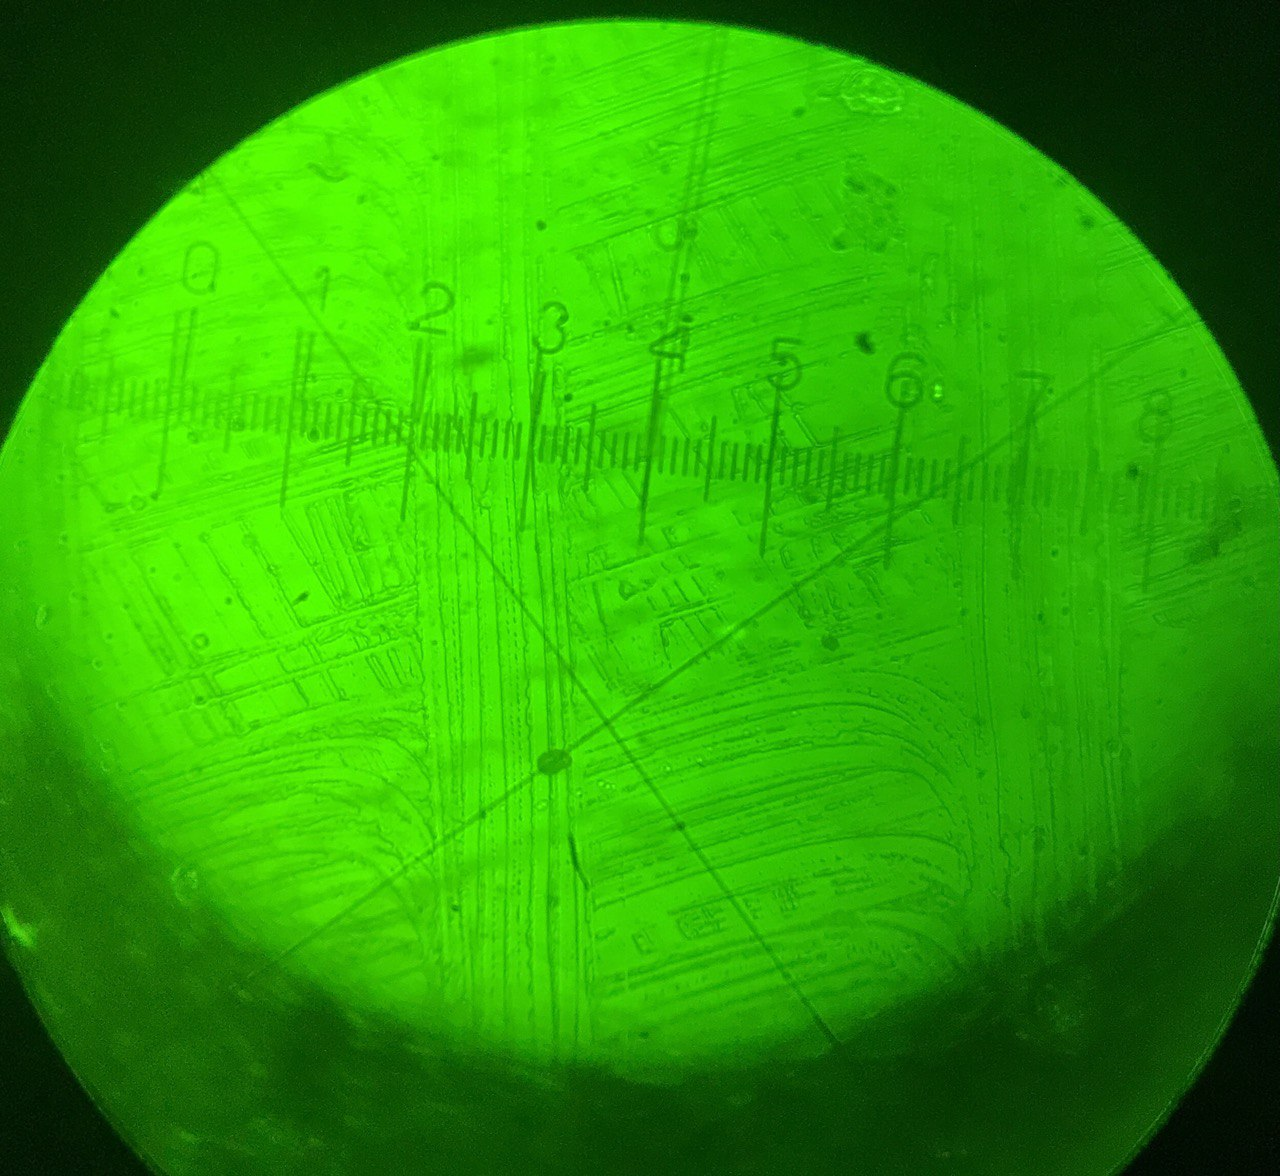
\includegraphics[width=0.25\linewidth]{линейка.png}
 \end{figure}

\begin{table}[h!]
\begin{tabular}{|lllll|}
\hline
\multicolumn{5}{|c|}{темные}                                                                                                                                                                  \\ \hline
\multicolumn{1}{|l|}{$m$} & \multicolumn{1}{l|}{$r_m, \text{ дел}$} & \multicolumn{1}{l|}{$r_m, \text{ мкм}$} & \multicolumn{1}{l|}{$r_m^2, \text{ мкм}^2$} & $\sigma_{r_{m}^2}, \text{ мкм}^2$ \\ \hline
\multicolumn{1}{|l|}{1}   & \multicolumn{1}{l|}{0,89}               & \multicolumn{1}{l|}{8,7}                & \multicolumn{1}{l|}{75,3}                   & 2,8                             \\ \hline
\multicolumn{1}{|l|}{2}   & \multicolumn{1}{l|}{1,2}                & \multicolumn{1}{l|}{11,7}               & \multicolumn{1}{l|}{136,9}                  & 2,8                             \\ \hline
\multicolumn{1}{|l|}{3}   & \multicolumn{1}{l|}{1,51}               & \multicolumn{1}{l|}{14,7}               & \multicolumn{1}{l|}{216,8}                  & 2,8                             \\ \hline
\multicolumn{1}{|l|}{4}   & \multicolumn{1}{l|}{1,75}               & \multicolumn{1}{l|}{17,1}               & \multicolumn{1}{l|}{291,1}                  & 2,8                             \\ \hline
\multicolumn{1}{|l|}{5}   & \multicolumn{1}{l|}{1,95}               & \multicolumn{1}{l|}{19,0}               & \multicolumn{1}{l|}{361,5}                  & 2,8                             \\ \hline
\multicolumn{1}{|l|}{6}   & \multicolumn{1}{l|}{2,17}               & \multicolumn{1}{l|}{21,2}               & \multicolumn{1}{l|}{447,6}                  & 2,8                             \\ \hline
\multicolumn{1}{|l|}{7}   & \multicolumn{1}{l|}{2,345}              & \multicolumn{1}{l|}{22,9}               & \multicolumn{1}{l|}{522,8}                  & 2,8                             \\ \hline
\multicolumn{1}{|l|}{8}   & \multicolumn{1}{l|}{2,47}               & \multicolumn{1}{l|}{24,1}               & \multicolumn{1}{l|}{580,0}                  & 3,4                             \\ \hline
\multicolumn{1}{|l|}{9}   & \multicolumn{1}{l|}{2,65}               & \multicolumn{1}{l|}{25,8}               & \multicolumn{1}{l|}{667,6}                  & 3,4                             \\ \hline
\multicolumn{1}{|l|}{10}  & \multicolumn{1}{l|}{2,81}               & \multicolumn{1}{l|}{27,4}               & \multicolumn{1}{l|}{750,6}                  & 3,4                             \\ \hline
\multicolumn{1}{|l|}{11}  & \multicolumn{1}{l|}{2,95}               & \multicolumn{1}{l|}{28,8}               & \multicolumn{1}{l|}{827,3}                  & 3,4                             \\ \hline
\multicolumn{1}{|l|}{12}  & \multicolumn{1}{l|}{3,08}               & \multicolumn{1}{l|}{30,0}               & \multicolumn{1}{l|}{901,8}                  & 3,4                             \\ \hline
\end{tabular}
\end{table}

\newpage

\begin{table}[h!]
\begin{tabular}{|lllll|}
\hline
\multicolumn{5}{|c|}{светлые}                                                                                                                                                                 \\ \hline
\multicolumn{1}{|l|}{$m$} & \multicolumn{1}{l|}{$r_m, \text{ дел}$} & \multicolumn{1}{l|}{$r_m, \text{ мкм}$} & \multicolumn{1}{l|}{$r_m^2, \text{ мкм}^2$} & $\sigma_{r_{m}^2}, \text{ мкм}^2$ \\ \hline
\multicolumn{1}{|l|}{1}   & \multicolumn{1}{l|}{3,77}               & \multicolumn{1}{l|}{6,7}                & \multicolumn{1}{l|}{45,3}                   & 2,8                             \\ \hline
\multicolumn{1}{|l|}{2}   & \multicolumn{1}{l|}{3,4}                & \multicolumn{1}{l|}{10,3}               & \multicolumn{1}{l|}{106,8}                  & 2,8                             \\ \hline
\multicolumn{1}{|l|}{3}   & \multicolumn{1}{l|}{3,08}               & \multicolumn{1}{l|}{13,5}               & \multicolumn{1}{l|}{181,0}                  & 2,8                             \\ \hline
\multicolumn{1}{|l|}{4}   & \multicolumn{1}{l|}{2,825}              & \multicolumn{1}{l|}{15,9}               & \multicolumn{1}{l|}{254,1}                  & 2,8                             \\ \hline
\multicolumn{1}{|l|}{5}   & \multicolumn{1}{l|}{2,62}               & \multicolumn{1}{l|}{17,9}               & \multicolumn{1}{l|}{321,8}                  & 2,8                             \\ \hline
\multicolumn{1}{|l|}{6}   & \multicolumn{1}{l|}{2,405}              & \multicolumn{1}{l|}{20,0}               & \multicolumn{1}{l|}{401,5}                  & 2,8                             \\ \hline
\multicolumn{1}{|l|}{7}   & \multicolumn{1}{l|}{2,21}               & \multicolumn{1}{l|}{21,9}               & \multicolumn{1}{l|}{481,3}                  & 2,8                             \\ \hline
\multicolumn{1}{|l|}{8}   & \multicolumn{1}{l|}{2,04}               & \multicolumn{1}{l|}{23,6}               & \multicolumn{1}{l|}{556,7}                  & 3,4                             \\ \hline
\multicolumn{1}{|l|}{9}   & \multicolumn{1}{l|}{1,885}              & \multicolumn{1}{l|}{25,1}               & \multicolumn{1}{l|}{630,3}                  & 3,4                             \\ \hline
\multicolumn{1}{|l|}{10}  & \multicolumn{1}{l|}{1,73}               & \multicolumn{1}{l|}{26,6}               & \multicolumn{1}{l|}{708,5}                  & 3,4                             \\ \hline
\multicolumn{1}{|l|}{11}  & \multicolumn{1}{l|}{1,59}               & \multicolumn{1}{l|}{28,0}               & \multicolumn{1}{l|}{783,0}                  & 3,4                             \\ \hline
\multicolumn{1}{|l|}{12}  & \multicolumn{1}{l|}{1,455}              & \multicolumn{1}{l|}{29,3}               & \multicolumn{1}{l|}{858,4}                  & 3,4                             \\ \hline
\end{tabular}
\end{table}

\noindent 3. Построим график $r_{m}^2(m)$ (см. ниже).

 \medskip


\noindent По наклону прямых найдем радиус кривизны линзы $R = 1,30 \pm 0,01 \text{ см}$. 

\medskip

\noindent 4. Найдем фокусное расстояние линзы и вычислим показатель преломления стекла по формуле $n = \frac{R}{F} + 1$.

$$F = 2,3 \text { см}$$
$$n = 1,567.$$


\subsection{Наблюдение биений}

\noindent Наблюдаем биения, между центрами четких систем разность $\Delta m = 16$ полос. Найдем разность длин волн для желтой и зеленой линий Hg ($ \lambda_\text{з} = 546 $ нм, $ \lambda_\text{ж} = 578  $ нм):

	$$(\Delta m + 1)\lambda_\text{з} = \Delta m \lambda_\text{ж}$$
	
	 $$\Delta \lambda = \dfrac{\lambda_\text{з}}{\Delta m} \approx 34 \text{ нм}.$$
 

\section{Вывод}

\noindent В ходе работы:

\medskip

\noindent - определен радиус кривизны линзы $R = 1,30 \pm 0,01 \text{ см}$;

\medskip

\noindent - вычислен показатель преломления стекла линзы ($n = 1,567$). Такой показатель преломления соответствует баритовому крону (БК-10);

\medskip

\noindent - найдена разность длин волн для желтой и зеленой линий Hg: $\Delta \lambda \approx 34 \text{ нм}.$ Это значение близко к табличному $\Delta \lambda_\text{табл} = 33 \text{ нм}.$

\section{График}

\begin{figure}[h!]
 	\centering 	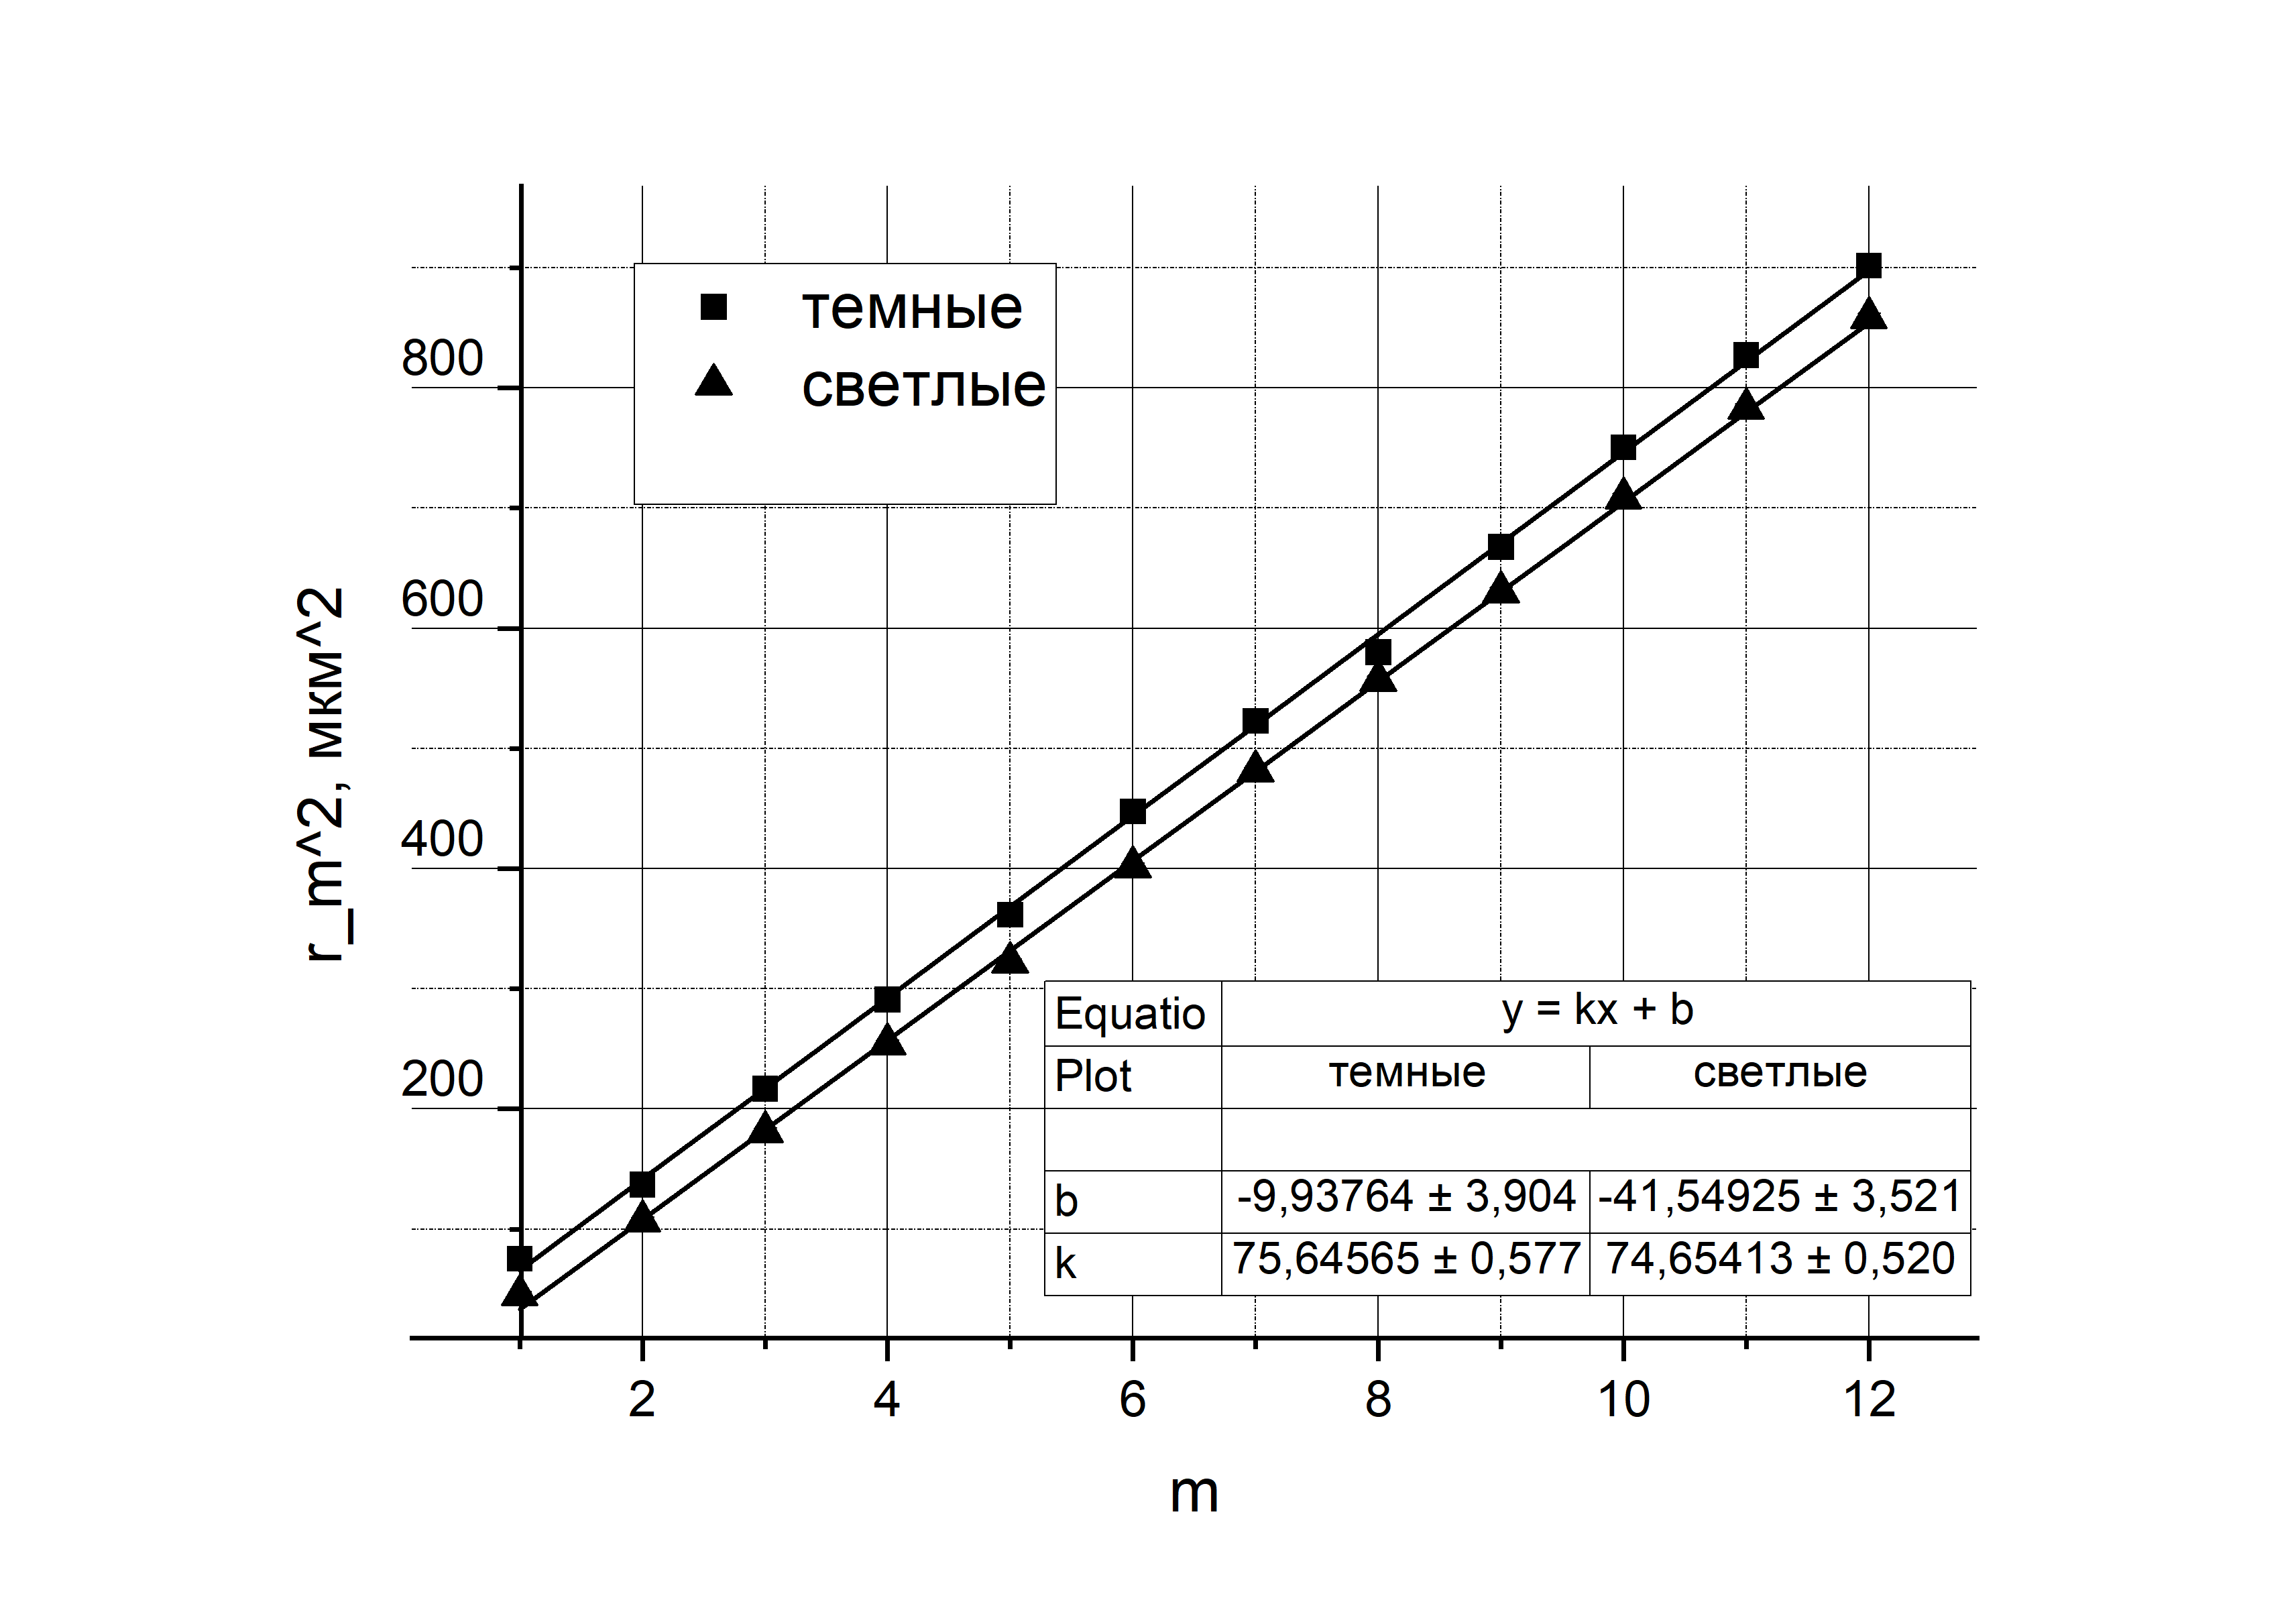
\includegraphics[width=0.8\linewidth]{график.png}
 \end{figure}
 

\end{document}